\documentclass[]{article}
\newcommand{\FileDepth}{../../..}
\usepackage[letterpaper, landscape, margin=0.5cm]{geometry}
\usepackage[T1]{fontenc}
\usepackage{textcomp}%Not strictly necessary, but gives \textmu command for "micro."
\usepackage{fancyhdr}
\usepackage{amsmath}
\usepackage{amssymb}
\usepackage{graphicx}
\usepackage{xcolor}
\usepackage{tikz}
\usetikzlibrary{calc}
\usepackage[shortlabels]{enumitem}
\usepackage{multicol}
\usepackage{vwcol}
\usepackage{hyperref}
\usepackage{wrapfig}
%opening
\newcommand{\SecType}{L}
\newcommand{\Week}{19}
\title{PH 211 Lecture \Week}
\author{Benjamin Bauml}
\date{Summer 2024}

\newcommand{\Purpose}{4}
\newcommand{\DefOnly}{0}

\input{\FileDepth/Formats/Assignment20240614.tex}
\usepackage[absolute]{textpos}
% This package relies on Assignment Format 2024-06-14 or later to work. It is recommended that the Purpose and DefOnly commands be given as such:
%\newcommand{\Purpose}{4}
%\newcommand{\DefOnly}{0}
% Activities need to be entered outside of the TeacherMargin and PresentSpace environments, otherwise they will be defined only locally. They can even go in the preamble.
\newenvironment{TeacherMargin}{\begin{textblock*}{10.8cm}(0.5cm,0.5cm)
\small}{\end{textblock*}
\hspace{0.1cm}}
\newenvironment{PresentSpace}{\begin{textblock*}{0.3cm}(26.85cm,9.35cm)
--
\end{textblock*}
\begin{textblock*}{15.6cm}(11.8cm,0.5cm)
\begin{Repurpose}{1}
\Large}{\end{Repurpose}
\end{textblock*}
\hspace{0.1cm}}

\newcommand{\FBDaxes}[4][2]{
	\begin{scope}[shift={(#2)},rotate=#3]
		% x-axis
		\draw[thick,->] (-#1,0) -- (#1,0);
		\node[anchor=west] at (#1,0) {$x$};
		% y-axis
		\draw[thick,->] (0,-#1) -- (0,#1);
		\node[anchor=south] at (0,#1) {$y$};
		\coordinate (#4) at (0,0);
	\end{scope}
}
\newcommand{\FBDvectorMA}[4]{
	\begin{scope}[shift={(#1)}]
		\coordinate (#4tip) at ({#2*cos(#3)},{#2*sin(#3)});
		\draw[ultra thick,blue,->] (#1) -- (#4tip);
	\end{scope}
}
\newcommand{\FBDvectorXY}[3]{
	\begin{scope}[shift={(#1)}]
		\coordinate (#3tip) at (#2);
		\draw[ultra thick,blue,->] (0,0) -- (#3tip);
	\end{scope}
}
\newcommand{\FBDdot}[1]{
	\filldraw[black] (#1) circle (3pt);
}
\newcommand{\FBDbox}[5][1]{
	\begin{scope}[shift={(#2)},rotate=#3]
		\filldraw[color=black,fill=white,thick] ({-#1/2},{#1/2}) -- ({-#1/2},{-#1/2}) -- ({#1/2},{-#1/2}) -- ({#1/2},{#1/2}) -- cycle;
		% Left side coordinates
		\coordinate (#4ltq) at ({-#1/2},{#1/4});
		\coordinate (#4lcent) at ({-#1/2},0);
		\coordinate (#4lbq) at ({-#1/2},{-#1/4});
		% right side coordinates
		\coordinate (#4rtq) at ({#1/2},{#1/4});
		\coordinate (#4rcent) at ({#1/2},0);
		\coordinate (#4rbq) at ({#1/2},{-#1/4});
		% top coordinates
		\coordinate (#4tlq) at ({-#1/4},{#1/2});
		\coordinate (#4tcent) at (0,{#1/2});
		\coordinate (#4trq) at ({#1/4},{#1/2});
		% bottom coordinates
		\coordinate (#4blq) at ({-#1/4},{-#1/2});
		\coordinate (#4bcent) at (0,{-#1/2});
		\coordinate (#4brq) at ({#1/4},{-#1/2});
		% corners
		\coordinate (#4tl) at ({-#1/2},{#1/2});
		\coordinate (#4tr) at ({#1/2},{#1/2});
		\coordinate (#4bl) at ({-#1/2},{-#1/2});
		\coordinate (#4br) at ({#1/2},{-#1/2});
		\node at (0,0) {#5};
	\end{scope}
}
% Renewing these commands so they can be used without preset color, and so a dot is placed at the tail of the vectors.
\renewcommand{\FBDvectorXY}[3]{
	\begin{scope}[shift={(#1)}]
		\coordinate (#3tip) at (#2);
		\draw[ultra thick,->] (0,0) -- (#3tip);
		\filldraw (0,0) circle (3pt);
	\end{scope}
}
\renewcommand{\FBDbox}[5][1]{
	\begin{scope}[shift={(#2)},rotate=#3]
		\filldraw[fill=white,thick] ({-#1/2},{#1/2}) -- ({-#1/2},{-#1/2}) -- ({#1/2},{-#1/2}) -- ({#1/2},{#1/2}) -- cycle;
		% Left side coordinates
		\coordinate (#4ltq) at ({-#1/2},{#1/4});
		\coordinate (#4lcent) at ({-#1/2},0);
		\coordinate (#4lbq) at ({-#1/2},{-#1/4});
		% right side coordinates
		\coordinate (#4rtq) at ({#1/2},{#1/4});
		\coordinate (#4rcent) at ({#1/2},0);
		\coordinate (#4rbq) at ({#1/2},{-#1/4});
		% top coordinates
		\coordinate (#4tlq) at ({-#1/4},{#1/2});
		\coordinate (#4tcent) at (0,{#1/2});
		\coordinate (#4trq) at ({#1/4},{#1/2});
		% bottom coordinates
		\coordinate (#4blq) at ({-#1/4},{-#1/2});
		\coordinate (#4bcent) at (0,{-#1/2});
		\coordinate (#4brq) at ({#1/4},{-#1/2});
		% corners
		\coordinate (#4tl) at ({-#1/2},{#1/2});
		\coordinate (#4tr) at ({#1/2},{#1/2});
		\coordinate (#4bl) at ({-#1/2},{-#1/2});
		\coordinate (#4br) at ({#1/2},{-#1/2});
		\node at (0,0) {#5};
	\end{scope}
}
\newcommand{\Longbox}[5][1]{
	\begin{scope}[shift={(#2)},rotate=#3]
		\filldraw[fill=white,thick] (-2.8,{#1/2}) -- (-2.8,{-#1/2}) -- ({#1/2},{-#1/2}) -- ({#1/2},{#1/2}) -- cycle;
		% Left side coordinates
		\coordinate (#4ltq) at (-2.8,{#1/4});
		\coordinate (#4lcent) at (-2.8,0);
		\coordinate (#4lbq) at (-2.8,{-#1/4});
		% right side coordinates
		\coordinate (#4rtq) at ({#1/2},{#1/4});
		\coordinate (#4rcent) at ({#1/2},0);
		\coordinate (#4rbq) at ({#1/2},{-#1/4});
		% top coordinates
		\coordinate (#4tlq) at ({-#1/4},{#1/2});
		\coordinate (#4tcent) at (0,{#1/2});
		\coordinate (#4trq) at ({#1/4},{#1/2});
		% bottom coordinates
		\coordinate (#4blq) at ({-#1/4},{-#1/2});
		\coordinate (#4bcent) at (0,{-#1/2});
		\coordinate (#4brq) at ({#1/4},{-#1/2});
		% corners
		\coordinate (#4tl) at (-2.8,{#1/2});
		\coordinate (#4tr) at ({#1/2},{#1/2});
		\coordinate (#4bl) at (-2.8,{-#1/2});
		\coordinate (#4br) at ({#1/2},{-#1/2});
		\node at (0,0) {#5};
	\end{scope}
}
%\newcommand{\MVec}[3][0]{%Creates a momentum vector of length #3 centered at #2 and rotated #1 degrees counterclockwise.
	\begin{scope}[rotate=#1,shift={(#2)}]
		\draw[->,thick] ({-#3/2},0) -- ({#3/2},0);
	\end{scope}
}
\newcommand{\MDot}[1]{%Creates a dot at #1 to represent a zero vector.
	\filldraw (#1) circle (1pt);
}
\newcommand{\MVDRows}[2][4.5]{%Creates the rows (initial, delta, final) of a momentum vector diagram. The optional argument determines the width of the table, and defaults to a good length for three columns (two objects and the total system). The non-optional argument gives a coordinate name (not displayed) to the diagram.
	\begin{scope}
		%\draw[thick] (0,5.5) -- (0,0);
		\draw[thick] (-1,4.5) -- (#1,4.5);
		\node at (-0.5,3.75) {$\vec{p}_{i}$};
		\draw[thick] (-1,3) -- (#1,3);
		\node at (-0.5,2.25) {$\Delta\vec{p}$};
		\draw[thick] (-1,1.5) -- (#1,1.5);
		\node at (-0.5,0.75) {$\vec{p}_{f}$};
		\coordinate (#2) at (0,5);
	\end{scope}
}
\newcommand{\MVDCol}[4][0.75]{%Creates a column for an object in a momentum vector diagram. The first (non-optional) argument is the coordinate name (not displayed) of the column, while the second is the displayed column header. The first argument also names the three entries down the column. The third argument anchors the column, so it should either be the coordinate name of the MVD (for the first column) or the coordinate name of the previous column. The optional argument indicates how far the center of the column should be from the previous column's edge, and defaults to 0.75.
	\begin{scope}[shift={(#4)}]
		\node at (#1,0) {#3};
		%\draw[thick] ({#1*2},0.5) -- ({#1*2},-5);
		\draw[thick] (0,0.5) -- (0,-5);
		\coordinate (#2init) at (#1,-1.25);
		\coordinate (#2delt) at (#1,-2.75);
		\coordinate (#2fin) at (#1,-4.25);
		\coordinate (#2) at ({#1*2},0);
	\end{scope}
}

%\input{\FileDepth/Activities/Activity_One/Activity_One.tex}
%\input{\FileDepth/Activities/Activity_Two/Activity_Two.tex}

\begin{document}
\begin{TeacherMargin}
\noindent It is often asserted that energy is always conserved, meaning that energy cannot be created or destroyed within the universe as a whole. \\

\noindent To be more exact and use the idea of energy conservation more practically, we should pick a system and look to the work energy theorem ($W_{\text{net,ext}}=\Delta E_{\text{total}}$) to tell us if energy is conserved for that system. If $W_{\text{net,ext}}=0$, then the energy of the system is conserved, and we can use energy conservation methods to analyze the system. \\

\noindent Assuming that the universe is a closed system, interacting with nothing outside of it, then our more exact idea of energy conservation implies that energy is indeed always conserved on a universal scale.
\end{TeacherMargin}
\begin{PresentSpace}
\begin{center}
	\huge Lecture \Week: Energy Conservation
\end{center}
\vspace{0.5cm}
\underline{Warm-Up Activity} \\
When can we say that energy is conserved?
\end{PresentSpace}
\newpage
\begin{TeacherMargin}
\noindent For this activity, I will identify the points of contact for forces on my free-body diagrams, which will violate our normal FBD conventions.
\begin{center}
	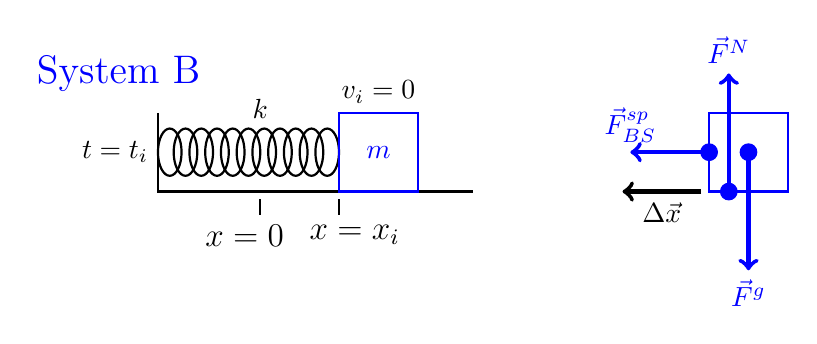
\begin{tikzpicture}
		\begin{scope}[shift={(0,0)}]
			\node[blue] at (-0.5,1.5) {\Large System B};
			\node[anchor=east] at (0,0.5) {$t=t_{i}$};
			\draw[thick] (0,1) -- (0,0) -- (4,0);
			\foreach \s in {0,1,2,3,4,5,6,7,8,9,10}
			\draw[thick] (\s*0.2+0.15,0.5) circle (0.15 and 0.3);
			\node[anchor=south] at (1.3,0.8) {$k$};
			\draw[thick,blue,shift={(2.3,0)}] (0,0) -- (0,1) -- (1,1) -- (1,0) -- cycle;
			\node[blue] at (2.8,0.5) {$m$};
			\node[anchor=south] at (2.8,1) {$v_{i}=0$};
			\draw[thick] (1.3,-0.1) -- (1.3,-0.3) node[anchor=north,shift={(-0.2,0)}] {\large$x=0$};
			\draw[thick] (2.3,-0.1) -- (2.3,-0.3) node[anchor=north,shift={(0.2,0)}] {\large$x=x_{i}$};
		\end{scope}
		\begin{scope}[shift={(7.5,0.5)},blue]
			\FBDbox{0,0}{0}{SysB}{}
			\FBDvectorXY{SysBlcent}{-1,0}{FSP}
			\node[anchor=south] at (FSPtip) {$\vec{F}^{sp}_{BS}$};
			\FBDvectorXY{SysBblq}{0,1.5}{FN}
			\node[anchor=south] at (FNtip) {$\vec{F}^{N}$};
			\FBDvectorXY{0,0}{0,-1.5}{FG}
			\node[anchor=north] at (FGtip) {$\vec{F}^{g}$};
			\draw[ultra thick,black,->] (-0.6,-0.5) -- (-1.1,-0.5) node[anchor=north] {$\Delta\vec{x}$} -- (-1.6,-0.5);
		\end{scope}
	\end{tikzpicture}
\end{center}
\begin{itemize}
	\item $W^{g}=0$ and $W^{N}=0$
	\begin{itemize}
		\item The points of contact for $F^{g}$ and $F^{N}$ are moving, but the forces are perpendicular to the displacement, so the work is zero.
	\end{itemize}
	\item $W^{sp}>0$
	\begin{itemize}
		\item The spring pulls to the left, in the direction of the displacement of its point of contact.
	\end{itemize}
\end{itemize}
\begin{center}
	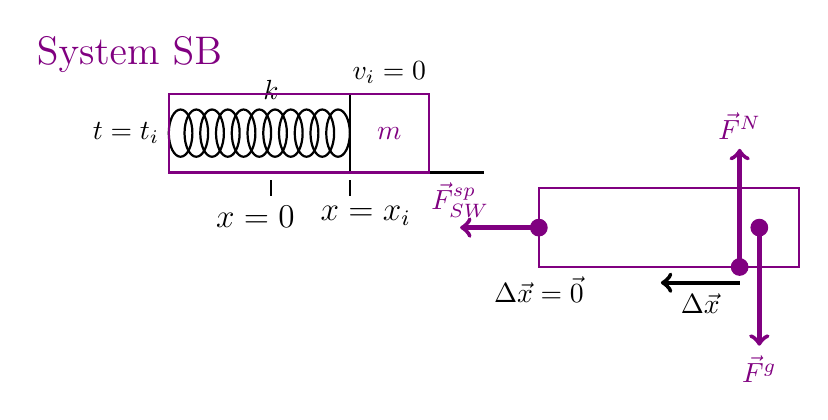
\begin{tikzpicture}
		\begin{scope}[shift={(0,0)}]
			\node[violet] at (-0.5,1.5) {\Large System SB};
			\node[anchor=east] at (0,0.5) {$t=t_{i}$};
			\draw[thick] (0,1) -- (0,0) -- (4,0);
			\foreach \s in {0,1,2,3,4,5,6,7,8,9,10}
			\draw[thick] (\s*0.2+0.15,0.5) circle (0.15 and 0.3);
			\node[anchor=south] at (1.3,0.8) {$k$};
			\draw[thick,shift={(2.3,0)}] (0,0) -- (0,1) -- (1,1) -- (1,0) -- cycle;
			\draw[thick,violet] (0,0) rectangle (3.3,1);
			\node[violet] at (2.8,0.5) {$m$};
			\node[anchor=south] at (2.8,1) {$v_{i}=0$};
			\draw[thick] (1.3,-0.1) -- (1.3,-0.3) node[anchor=north,shift={(-0.2,0)}] {\large$x=0$};
			\draw[thick] (2.3,-0.1) -- (2.3,-0.3) node[anchor=north,shift={(0.2,0)}] {\large$x=x_{i}$};
		\end{scope}
		\begin{scope}[shift={(7.5,-0.7)},violet]
			\Longbox{0,0}{0}{SysSB}{}
			\FBDvectorXY{SysSBlcent}{-1,0}{FSP}
			\node[anchor=south] at (FSPtip) {$\vec{F}^{sp}_{SW}$};
			\node[anchor=north,black] at (SysSBbl) {$\Delta\vec{x}=\vec{0}$};
			\FBDvectorXY{SysSBblq}{0,1.5}{FN}
			\node[anchor=south] at (FNtip) {$\vec{F}^{N}$};
			\FBDvectorXY{0,0}{0,-1.5}{FG}
			\node[anchor=north] at (FGtip) {$\vec{F}^{g}$};
			\draw[ultra thick,black,->] (-0.25,-0.7) -- (-0.75,-0.7) node[anchor=north] {$\Delta\vec{x}$} -- (-1.25,-0.7);
		\end{scope}
	\end{tikzpicture}
\end{center}
\begin{itemize}
\item $W^{g}=0$ and $W^{N}=0$
\begin{itemize}
	\item Same as before.
\end{itemize}
\item $W^{sp}=0$
\begin{itemize}
	\item The work done on the spring by the wall is zero, as the point of contact at the stationary wall undergoes no displacement.
\end{itemize}
\end{itemize}
\begin{center}
	\Large
	\begin{tabular}{c||c|c|c||c|c|c}
		System & \multicolumn{3}{c||}{B} & \multicolumn{3}{c}{SB} \\ \hline
		Forces & $\vec{F}^{g}$ & $\vec{F}^{N}$ & $\vec{F}^{sp}$ & $\vec{F}^{g}$ & $\vec{F}^{N}$ & $\vec{F}^{sp}$ \\ \hline
		Displacements & $\Delta\vec{x}$ & $\Delta\vec{x}$ & $\Delta\vec{x}$ & $\Delta\vec{x}$ & $\Delta\vec{x}$ & 0 \\ \hline
		Works & 0 & 0 & $W^{sp}$ & 0 & 0 & 0
	\end{tabular}
\end{center}
\end{TeacherMargin}
\begin{PresentSpace}
\vspace{-10pt}
\section*{L\Week-1: Block on a Spring -- Forces}
\vspace{-10pt}
\begin{itemize}
	\large
	\item A block of mass $m$ on a level, frictionless surface is attached to an ideal, massless spring of constant $k$ that is initially stretched.
	\item At time $t_{i}$, the block is \textbf{released from rest} at $x=x_{i}$.
	\item At time $t_{f}$, the block reaches $x=0$ moving to \\
	the left with speed $v_{f}$.
	\item System B consists of the block alone.
	\item System SB consists of the spring and the block.
	\item For the interval from $t_{i}$ to $t_{f}$ (for each system):
	\begin{enumerate}[(1)]
		\normalsize
		\item List all external forces acting on the system.
		\item Identify the point of contact associated with each force.
		\item Draw a vector to indicate the \textbf{displacement} associated with each force.
		\item Determine if the work done by \textbf{each force} is positive, negative, or zero.
	\end{enumerate}
	\item What do you want to remember about this situation for future problems?
\end{itemize}
\end{PresentSpace}
\begin{textblock*}{5cm}(22cm,2cm)
\begin{center}
	\Large
	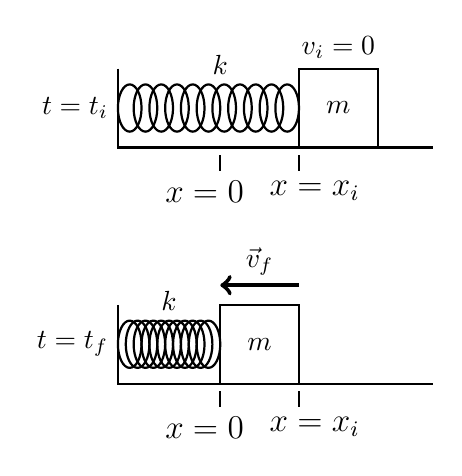
\begin{tikzpicture}
		\begin{scope}[shift={(0,-3)}]
			\node[anchor=east] at (0,0.5) {$t=t_{f}$};
			\draw[thick] (0,1) -- (0,0) -- (4,0);
			\foreach \s in {0,1,2,3,4,5,6,7,8,9,10}
			\draw[thick] (\s*0.1+0.15,0.5) circle (0.15 and 0.3);
			\node[anchor=south] at (0.65,0.8) {$k$};
			\draw[thick,shift={(1.3,0)}] (0,0) -- (0,1) -- (1,1) -- (1,0) -- cycle;
			\node at (1.8,0.5) {$m$};
			\draw[ultra thick,<-,shift={(1.3,0)}] (0,1.25) -- (0.5,1.25) -- (1,1.25);
			\node[anchor=south] at (1.8,1.25) {$\vec{v}_{f}$};
			\draw[thick] (1.3,-0.1) -- (1.3,-0.3) node[anchor=north,shift={(-0.2,0)}] {\large$x=0$};
			\draw[thick] (2.3,-0.1) -- (2.3,-0.3) node[anchor=north,shift={(0.2,0)}] {\large$x=x_{i}$};
		\end{scope}
		\begin{scope}[shift={(0,0)}]
			\node[anchor=east] at (0,0.5) {$t=t_{i}$};
			\draw[thick] (0,1) -- (0,0) -- (4,0);
			\foreach \s in {0,1,2,3,4,5,6,7,8,9,10}
			\draw[thick] (\s*0.2+0.15,0.5) circle (0.15 and 0.3);
			\node[anchor=south] at (1.3,0.8) {$k$};
			\draw[thick,shift={(2.3,0)}] (0,0) -- (0,1) -- (1,1) -- (1,0) -- cycle;
			\node at (2.8,0.5) {$m$};
			\node[anchor=south] at (2.8,1) {$v_{i}=0$};
			\draw[thick] (1.3,-0.1) -- (1.3,-0.3) node[anchor=north,shift={(-0.2,0)}] {\large$x=0$};
			\draw[thick] (2.3,-0.1) -- (2.3,-0.3) node[anchor=north,shift={(0.2,0)}] {\large$x=x_{i}$};
		\end{scope}
	\end{tikzpicture}
\end{center}
\end{textblock*}
\newpage
\begin{TeacherMargin}
\begin{center}
	\Large
	\begin{tabular}{c|c|c|c}
		System & {\color{blue}B} & {\color{violet}SB} & \\ \hline
		$W_{\text{net,ext}}$ & {\color{blue}$+$} & {\color{violet}0} & \parbox{3cm}{\small For B, there is net external work, but for SB, there is not. This follows from the previous activity.} \\ \hline
		$\Delta E_{\text{total}}$ & {\color{blue}$+$} & {\color{violet}0} & \parbox{3cm}{\small By the work-energy theorem, $\Delta E_{\text{total}}=W_{\text{net,ext}}$.} \\ \hline
		$\Delta K$ & {\color{blue}$+$} & {\color{violet}$+$} & \parbox{3cm}{\small The block starts at rest and ends with nonzero speed, so it must have gained kinetic energy, regardless of our choice of system.} \\ \hline
		$\Delta U$ & {\color{blue}0} & {\color{violet}$-$} & 
	\end{tabular}
\end{center}
{\color{blue} A block by itself that cannot change elevation can only have kinetic energy. It has no way of storing energy (no potential).}

\noindent{\color{violet} Without external work, the $\Delta K$ in SB must come from somewhere, and $\Delta E_{\text{total}}=0$, so there must be energy stored in the system that is transformed into kinetic energy. By putting the spring in the system, the system can now store potential energy.}
\end{TeacherMargin}
\begin{PresentSpace}
\vspace{-10pt}
\section*{L\Week-2: Block on a Spring -- Energy}
\vspace{-10pt}
\begin{itemize}
	\large
	\item A block of mass $m$ on a level, frictionless surface is attached to an ideal, massless spring of constant $k$ that is initially stretched.
	\item At time $t_{i}$, the block is \textbf{released from rest} at $x=x_{i}$.
	\item At time $t_{f}$, the block reaches $x=0$ moving to \\
	the left with speed $v_{f}$.
	\item System B consists of the block alone.
	\item System SB consists of the spring and the block.
	\item For the interval from $t_{i}$ to $t_{f}$ (for each system):
	\begin{enumerate}[(1)]
		\normalsize
		\item Determine if the \textbf{net external work} is positive, \\
		negative, or zero (based on L19-1).
		\item Determine if the \textbf{change in total energy} is positive, negative, or zero.
		\item Determine if the \textbf{change in kinetic energy} is positive, negative, or zero.
		\item Determine if the \textbf{change in potential energy} is positive, negative, or zero.
	\end{enumerate}
	\item What is different about the two systems?
\end{itemize}
\end{PresentSpace}
\begin{textblock*}{5cm}(22cm,2cm)
\begin{center}
	\Large
	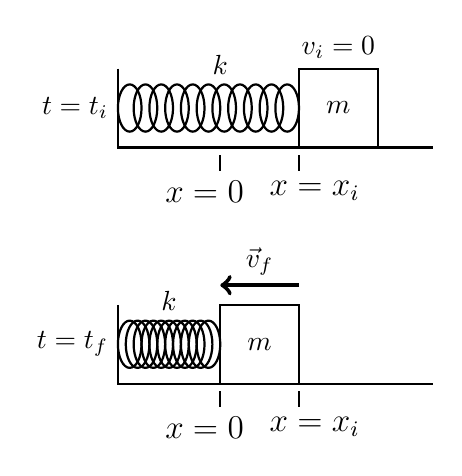
\begin{tikzpicture}
		\begin{scope}[shift={(0,-3)}]
			\node[anchor=east] at (0,0.5) {$t=t_{f}$};
			\draw[thick] (0,1) -- (0,0) -- (4,0);
			\foreach \s in {0,1,2,3,4,5,6,7,8,9,10}
			\draw[thick] (\s*0.1+0.15,0.5) circle (0.15 and 0.3);
			\node[anchor=south] at (0.65,0.8) {$k$};
			\draw[thick,shift={(1.3,0)}] (0,0) -- (0,1) -- (1,1) -- (1,0) -- cycle;
			\node at (1.8,0.5) {$m$};
			\draw[ultra thick,<-,shift={(1.3,0)}] (0,1.25) -- (0.5,1.25) -- (1,1.25);
			\node[anchor=south] at (1.8,1.25) {$\vec{v}_{f}$};
			\draw[thick] (1.3,-0.1) -- (1.3,-0.3) node[anchor=north,shift={(-0.2,0)}] {\large$x=0$};
			\draw[thick] (2.3,-0.1) -- (2.3,-0.3) node[anchor=north,shift={(0.2,0)}] {\large$x=x_{i}$};
		\end{scope}
		\begin{scope}[shift={(0,0)}]
			\node[anchor=east] at (0,0.5) {$t=t_{i}$};
			\draw[thick] (0,1) -- (0,0) -- (4,0);
			\foreach \s in {0,1,2,3,4,5,6,7,8,9,10}
			\draw[thick] (\s*0.2+0.15,0.5) circle (0.15 and 0.3);
			\node[anchor=south] at (1.3,0.8) {$k$};
			\draw[thick,shift={(2.3,0)}] (0,0) -- (0,1) -- (1,1) -- (1,0) -- cycle;
			\node at (2.8,0.5) {$m$};
			\node[anchor=south] at (2.8,1) {$v_{i}=0$};
			\draw[thick] (1.3,-0.1) -- (1.3,-0.3) node[anchor=north,shift={(-0.2,0)}] {\large$x=0$};
			\draw[thick] (2.3,-0.1) -- (2.3,-0.3) node[anchor=north,shift={(0.2,0)}] {\large$x=x_{i}$};
		\end{scope}
	\end{tikzpicture}
\end{center}
\end{textblock*}
\newpage
\begin{TeacherMargin}
\begin{center}
	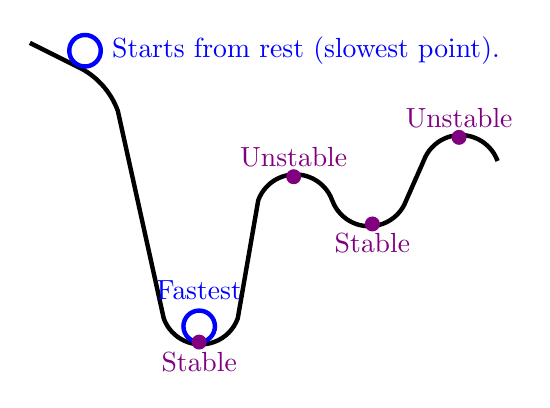
\begin{tikzpicture}
		\draw[ultra thick] (0,4) -- (0.6,3.7) arc (65:20:1) -- (1.7,0.5) arc (200:340:0.5) -- (2.9,2) arc (160:20:0.5) arc (200:340:0.5) -- (5,2.5) arc (160:20:0.5);
		\draw[ultra thick,blue] (0.7,3.9) circle (0.2) node[anchor=west,shift={(0.2,0)}] {Starts from rest (slowest point).};
		\draw[ultra thick,blue] (2.15,0.4) circle (0.2) node[anchor=south,shift={(0,0.2)}] {Fastest};
		\filldraw[violet] (2.15,0.2) circle (2.5pt) node[anchor=north] {Stable};
		\filldraw[violet] (3.35,2.3) circle (2.5pt) node[anchor=south] {Unstable};
		\filldraw[violet] (4.35,1.7) circle (2.5pt) node[anchor=north] {Stable};
		\filldraw[violet] (5.45,2.8) circle (2.5pt) node[anchor=south] {Unstable};
	\end{tikzpicture}
\end{center}
\begin{enumerate}[(1)]
	\item The ball will be moving fastest at the lowest point on the track, where the most potential energy has been transformed into kinetic energy.
	\item The ball will be moving slowest at the top of the track, where it starts with zero speed. \\
	It won't be going slowest at the two small peaks, but those will be local minima for its speed, as its kinetic energy will be at a local minimum in these places.
	\item There are stable equilibrium points at the bottoms of the two dips in the track. If the ball is placed slightly off of one of these points, it will want to fall downhill toward it.
	\item There are unstable equilibrium points at the tops of the two peaks on the track. If the ball is placed perfectly at one of these points, it will stay, but if it is placed slightly off of one of these points, it will want to fall downhill away from it.
	\item Since $U_{g}=mgh$, the graph will have the same shape as the physical track. We can choose the put the origin anywhere, but for simplicity, let us set $x=0$ at the left side of the track to make all positions on the track positive, and let us set $U_{g}=0$ at the bottom of the lowest point of the track to make all energy on the track positive.
\end{enumerate}
\begin{center}
	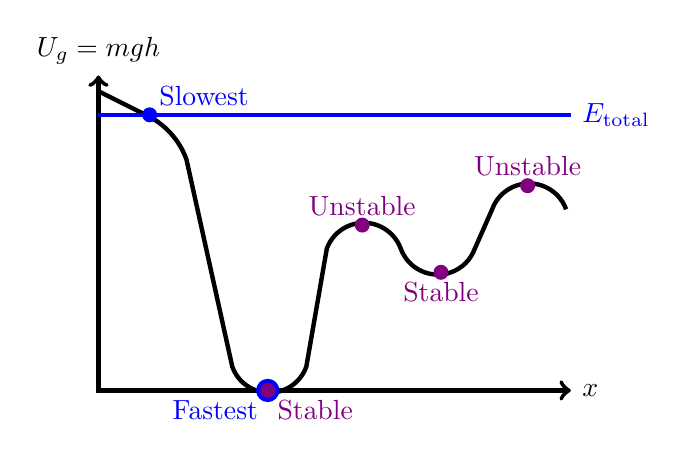
\begin{tikzpicture}
		\draw[ultra thick,<->] (0,4.2) node[anchor=south] {$U_{g}=mgh$} -- (0,0.2) -- (6,0.2) node[anchor=west] {$x$};
		\draw[ultra thick] (0,4) -- (0.6,3.7) arc (65:20:1) -- (1.7,0.5) arc (200:340:0.5) -- (2.9,2) arc (160:20:0.5) arc (200:340:0.5) -- (5,2.5) arc (160:20:0.5);
		\filldraw[blue] (0.65,3.7) circle (2.5pt) node[anchor=south west] {Slowest};
		\draw[ultra thick,blue] (0,3.7) -- (6,3.7) node[anchor=west] {$E_{\text{total}}$};
		%\draw[ultra thick,blue] (2.15,0.4) circle (0.2) node[anchor=south,shift={(0,0.2)}] {Fastest};
		\filldraw[blue] (2.15,0.2) circle (4pt) node[anchor=north east] {Fastest};
		\filldraw[violet] (2.15,0.2) circle (2.5pt) node[anchor=north west] {Stable};
		\filldraw[violet] (3.35,2.3) circle (2.5pt) node[anchor=south] {Unstable};
		\filldraw[violet] (4.35,1.7) circle (2.5pt) node[anchor=north] {Stable};
		\filldraw[violet] (5.45,2.8) circle (2.5pt) node[anchor=south] {Unstable};
	\end{tikzpicture}
\end{center}
\begin{enumerate}[(8)]
	\item Equilibrium occurs where the slope is zero: $\frac{\partial U_{g}}{\partial x} = 0$ (which is where the force from that potential is zero). \\
	Stable equilibrium occurs where the graph is concave up: $\frac{\partial^{2} U_{g}}{\partial x^{2}} > 0$. \\
	Unstable equilibrium occurs where it is concave down: $\frac{\partial^{2} U_{g}}{\partial x^{2}} < 0$.
\end{enumerate}
\end{TeacherMargin}
\begin{PresentSpace}
\vspace{-10pt}
\section*{L\Week-3: Undulant Track}
\vspace{-10pt}
\large
Consider the ball that can roll on the track in the center of the room. Ignore friction and air resistance. The ball starts from rest at the top of the track. Use the apparatus to see how the ball moves.
\begin{enumerate}[(1)]
	\item At what point will the ball be moving the fastest? How do you know?
	\item At what point will the ball be moving the slowest? How do you know?
	\item Are there any stable equilibrium points? If so, then where are they located?
	\item Are there any unstable equilibrium points? If so, then where are they located?
	\item Make a graph of the gravitational potential energy of the ball vs. the horizontal position. Remember to define the origin.
	\item On the same set of axes, make a graph of the total mechanical energy of the ball vs. horizontal position. Assume that the ball starts from rest.
	\item Where are the points determined previously for questions 1 through 4 above located on the graph?
	\item How can stable and unstable equilibrium points be defined in terms of the graph of potential energy vs. horizontal position?
\end{enumerate}
\end{PresentSpace}
\end{document}